\chapter{Результаты} 
\label{results}

В данной главе будет описана обучающая выборка с русской музыкой, на которой были поставлены эксперименты. 
Также будут приведены результаты этих экспериментов: по сопоставлению тегов треку 
и по поиску релевантных треков по заданному тегу. Будет проведено сравнение существующих алгоритмов
автоматического тегирования с предложенной модификацией.

\section{Построение обучающей выборки с русской музыкой}

Наша обучающая выборка русской музыки составлена экспертным путем из 613 треков разных исполнителей над словарем из 48 тегов. 
В качестве тегов брались названия радиостанций музыкального сервиса социальной сети ``Одноклассники''.
В таблице \ref{tab:rus_dataset} приведены краткие характеристики выборки, а в таблице \ref{tab:tags} перечислены исползуемые теги.
\begin{table}[ht]
\centering
\captionsetup{justification=centering}
\caption{Параметры обучающей выборки русской музыки.}
\label{tab:rus_dataset}
\begin{tabular}{ |c c c p{5cm}| }
  \hline    
  Треков & Тегов & Ср.число тегов на трек & Топ самых частых тегов \\  
  \hline    
  613 & 48 & $2.02$ & 
  Поп-музыка (386), Молодежная музыка(100), Шансон(99), Ретро(59), Рок(56) \\  
  \hline    
\end{tabular}
\end{table}

\begin{table}[ht]
\centering
\captionsetup{justification=centering}
\caption{Список тегов обучающей выборки русской музыки.}
\label{tab:tags}
\begin{tabular}{ |p{15cm}| }
  \hline    
  \emph{Песни под гитару, Джаз, Дискотека 00-х, Дискотека 90-х, Дискотека 80-х, Електронная музыка,
Рэп, Социальный рэп, Музыка улиц, Классическая музыка, Песни без цензуры, Детские песни, R'n'B, Барды, Металл, Рок-н-ролл,
Молодежная музыка, Танцевальная музыка, Молодежный рок, Песни за жизнь, Поп-рок, Инструментальная музыка, Эстрадная музыка,
Диско, Этническая музыка, Рок, Авторская песня, Альтернативный рок, Романтическая музыка, Поп-музыка, Панк-рок,
Классика русского рока, Тяжелый металл, Хип-хоп, Застольная музыка, Панк, Фолк-рока, Песни про любовь, Фолк, Ретро.}\\
\hline    
\end{tabular}
\end{table}
Как можно видеть из таблиц, самый популярнй тег \ld ``поп-музыка'', и в среднем приходится по два тега на трек.
Также на каждого исполнителя, присутствующего в данной выборке, было подготовлено от 7 до 10 треков, не присутствующих в выборке.

\section{Выбор параметров алгоритмов}

Результаты работы алгоритма автоматического тегирования зависят от различных параметров:
\begin{enumerate}
 \item использование высокоуровневых (high-level) характеристических признаков;
 \item количество информации, сохраняемое после уменьшения размерности данных (PCA covered variance);
 \item метрика измерения расстояния;
 \item количество ближайших соседей;
\end{enumerate}

В своей работе Mohamed Sordo исследовал влияние различных параметров на результат работы алгоритмов ближайших соседей 
и сравнил результаты с другими алгоритмами. В таблице \ref{tab:old_algo_settings} приведены параметры настройки алгоритмов, используемых в той работе.
\begin{table}[ht]
\centering
\captionsetup{justification=centering}
\caption{Список различных параметров, используемых в работе Mohamed Sordo для настройки алгоритмов ближайших соседей.}
\label{tab:old_algo_settings}
\begin{tabular}{ p{5cm}  p{4cm} }
  \hline    
  Параметр & Значения \\
  \hline    
  PCA covered variance & $75\%, 80\%, 85\%, 90\%, 100\% $ \\
  High-level хар.признаки & Да, Нет \\
  Метрика расстояния & евклидова, косинусная, взвешенная евклидова, Махалонобиса\\
  Кол-во ближайших соседей ($k$) & $1, \ldots, 20$ \\
  \hline    
\end{tabular}
\end{table}

В результате исследований Mohamed Sordo было отмечено, что:
\begin{enumerate}
 \item Наилучшие результаты алгоритмов были получены на больших значениях $k$ ($k = 18, 19, 20$, причем результаты при этих $k$ отличаются незначительно).
 \item Начиная с $75\%$ покрытой дисперсии в алгоритме PCA, прирост в качестве тегирования был незначительный (по сравнению с сопутствующим увеличением размерности пространства).
 При таком покрытии дисперсии размерность пространства уменишилась до ~30.
 \item Использование high-level хар.признаков дает заменый прирост в качесте тегирования.
 \item Евклидова и косинустная метрики показывают более хорошие результаты.
\end{enumerate}

Так как целью данной работы является улучшение существующих алгоритмов автоматического тегирования, зафиксируем параметры, при которых существующие подходы дают наилучшие результаты, 
и сравним их с результатами использования нового подохода. Также, следуюя примеру Mohamed Sordo, рассмотрим результаты алгоритма 2-NN для сравнения с алгоритмом CBDC.
В итоге имеем следующие параметры алгоритмов автоматического тегирования:
\begin{table}[ht]
\centering
\captionsetup{justification=centering}
\caption{Список различных параметров, используемых в данном исследовании для настройки алгоритмов ближайших соседей.}
\label{tab:new_algo_settings}
\begin{tabular}{ p{5cm}  p{4cm} }
  \hline    
  Параметр & Значения \\
  \hline    
  PCA covered variance & $75\%$ \\
  High-level хар.признаки & Да \\
  Метрика расстояния & евклидова, косинусная \\
  Кол-во ближайших соседей ($k$) & $2, 18$ \\
  \hline    
\end{tabular}
\end{table}

\section{Эксперимент по сопоставлению тегов треку}

В данном эксперименте мы фокусируемся на задаче сопоставления тегов треку. Для оценки качества тегирования и сравнения результатов использовались такие величины, как
точность (precision), полнота (recall) и F-мера (F-measure). Подсчет производился кросс-валидацией, где $\frac{1}{10}$ часть обучающей выборки бралась для тестирования, а остальная \ld для тренировки.
Каждая из них считалась в двух вариантах \ld относительно трека (per-song) и относительно тега (per-word).
Каждому треку сопоставлялось 2 тега, что является средним числом тегов на трек в обучающей выборке. Причем каждый из последних вариантов считался в двух метриках \ld косинусная (cos) и евклидова (euc).

Для фильтрации тегов использовалось три стратегии, описанные в главе \ref{chapter1}:
\begin{enumerate}
 \item фиксирование двух самых частых тегов (fir);
 \item введение ограничивающего порога (thr);
 \item использование функции взвешивания (wei).
\end{enumerate}
Во втором случае в качестве порога бралась величина $thresold = 0.250$. В третьем случае в качесвте функции взвешивания бралась функция из главы \ref{chapter1}.

Рассмотрим полученные результаты. В таблицах \ref{tab:annotation_persong} и \ref{tab:annotation_perword} приведены результаты относительно трека и тега соответственно.
На рисунках \ref{pic:persong} и \ref{pic:perword} приведены гистограммы, иллюстрирующие значения из соответствующих таблиц.
\begin{table}[ht]
\centering
\captionsetup{justification=centering}
\caption{Таблица с результатами запуска модификаций алгоритмов 2-NN, 18-NN и CBDC с применением перехода к исполнителю и без, 
persong-статистика, thresold = 0.250. ПИ \ld переход к исполнителю.}
\label{tab:annotation_persong}
\begin{tabular}{l c c ccc}
\hline\hline
 Алгоритм & Метрика & ПИ & Precision & Recall & F-measure
\\ [0.5ex]
    \hline
   
    & & нет&$0.418$ & $0.452$ & $0.423$ \\[-1.5ex]
    \raisebox{1ex}{2NN(fir)} & \raisebox{1ex}{cos}
    & да &$0.607$ & $0.724$ & $0.644$ \\[2ex]

    & & нет&$0.549$ & $0.645$ & $0.580$ \\[-1.5ex]
    \raisebox{1ex}{18NN(fir)} & \raisebox{1ex}{cos}
    & да &$\textbf{0.623}$ & $\textbf{0.735}$ & $\textbf{0.660}$ \\[2ex]

    & & нет&$0.451$ & $0.464$ & $0.448$ \\[-1.5ex]
    \raisebox{1ex}{2NN(fir)} & \raisebox{1ex}{euc}
    & да &$0.574$ & $0.686$ & $0.610$ \\[2ex]

    & & нет&$0.516$ & $0.604$ & $0.545$ \\[-1.5ex]
    \raisebox{1ex}{18NN(fir)} & \raisebox{1ex}{euc}
    & да &$0.574$ & $0.686$ & $0.610$ \\[2ex]

    & & нет&$0.500$ & $0.587$ & $0.528$ \\[-1.5ex]
    \raisebox{1ex}{2NN(wei)} & \raisebox{1ex}{cos}
    & да &$0.615$ & $0.735$ & $0.654$ \\[2ex]

    & & нет&$0.533$ & $0.612$ & $0.558$ \\[-1.5ex]
    \raisebox{1ex}{18NN(wei)} & \raisebox{1ex}{cos}
    & да &$0.615$ & $0.735$ & $0.654$ \\[2ex]

    & & нет&$0.516$ & $0.555$ & $0.510$ \\[-1.5ex]
    \raisebox{1ex}{2NN(wei)} & \raisebox{1ex}{euc}
    & да &$0.582$ & $0.694$ & $0.619$ \\[2ex]

    & & нет&$0.516$ & $0.587$ & $0.534$ \\[-1.5ex]
    \raisebox{1ex}{18NN(wei)} & \raisebox{1ex}{euc}
    & да &$0.582$ & $0.694$ & $0.619$ \\[2ex]

    & & нет&$0.246$ & $0.257$ & $0.231$ \\[-1.5ex]
    \raisebox{1ex}{CBDC} & \raisebox{1ex}{euc}
    & да &$0.287$ & $0.342$ & $0.304$ \\[2ex]

    & & нет&$0.303$ & $0.298$ & $0.291$ \\[-1.5ex]
    \raisebox{1ex}{CBDC} & \raisebox{1ex}{cos}
    & да &$0.377$ & $0.385$ & $0.368$ \\[2ex]
    
    & & нет&$0.386$ & $0.634$ & $0.465$ \\[-1.5ex]
    \raisebox{1ex}{2NN(thr)} & \raisebox{1ex}{cos}
    & да &$0.186$ & $0.917$ & $0.302$ \\[2ex]

    & & нет&$0.664$ & $0.634$ & $0.590$ \\[-1.5ex]
    \raisebox{1ex}{18NN(thr)} & \raisebox{1ex}{cos}
    & да &$0.378$ & $0.917$ & $0.478$ \\[2ex]

    & & нет&$0.442$ & $0.628$ & $0.500$ \\[-1.5ex]
    \raisebox{1ex}{2NN(thr)} & \raisebox{1ex}{euc}
    & да &$0.187$ & $0.910$ & $0.304$ \\[2ex]

    & & нет&$0.593$ & $0.628$ & $0.553$ \\[-1.5ex]
    \raisebox{1ex}{18NN(thr)} & \raisebox{1ex}{euc}
    & да &$0.405$ & $0.910$ & $0.507$ \\[2ex]

    \hline
\end{tabular}
\end{table}

\begin{figure}[h!]
\center{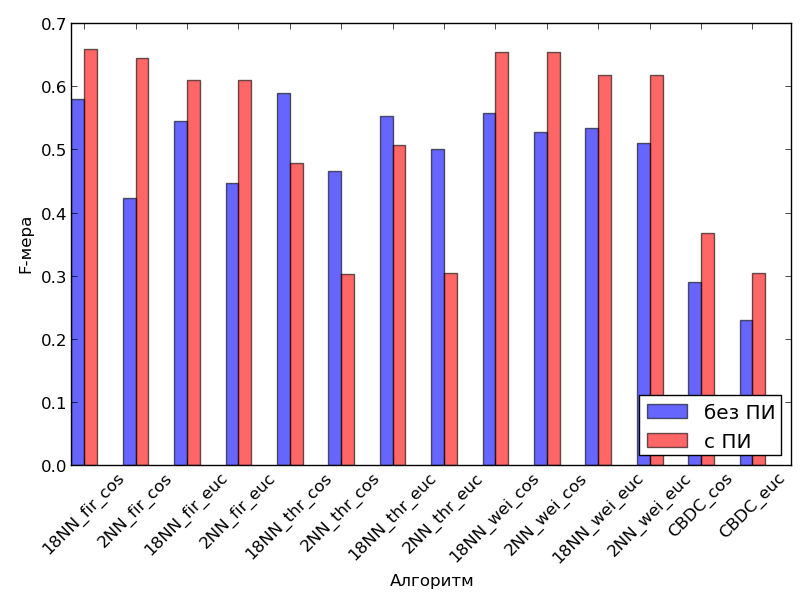
\includegraphics[width=170mm\textwidth]{persong.png}}
\caption{Гистограмма результатов запуска модификаций алгоритмов 2-NN, 18-NN и CBDC с применением перехода к исполнителю и без, 
persong-статистика, thresold = 0.250. ПИ \ld переход к исполнителю.}
\label{pic:persong}
\end{figure}

\begin{table}[ht]
\centering
\captionsetup{justification=centering}
\caption{Таблица с результатами запуска модификаций алгоритмов 2-NN, 18-NN и CBDC с применением перехода к исполнителю и без, perword-статистика, thresold = 0.250. ПИ \ld переход к исполнителю.}
\label{tab:annotation_perword}
\begin{tabular}{l c c ccc}
\hline\hline
 Алгоритм & Метрика & Исп.ПИ. & Precision & Recall & F-measure
\\ [0.5ex]
    \hline

    
    & & нет&$0.233$ & $0.306$ & $0.245$ \\[-1.5ex]
    \raisebox{1ex}{2NN(fir)} & \raisebox{1ex}{cos}
    & да &$0.309$ & $0.322$ & $0.315$ \\[2ex]

    & & нет&$0.236$ & $0.306$ & $0.245$ \\[-1.5ex]
    \raisebox{1ex}{18NN(fir)} & \raisebox{1ex}{cos}
    & да &$0.309$ & $0.322$ & $0.315$ \\[2ex]	

    & & нет&$0.205$ & $0.281$ & $0.236$ \\[-1.5ex]
    \raisebox{1ex}{2NN(fir)} & \raisebox{1ex}{euc}
    & да &$0.287$ & $0.308$ & $0.270$ \\[2ex]

    & & нет&$0.250$ & $0.281$ & $0.236$ \\[-1.5ex]
    \raisebox{1ex}{18NN(fir)} & \raisebox{1ex}{euc}
    & да &$0.287$ & $0.308$ & $0.270$ \\[2ex]

    & & нет&$0.223$ & $0.207$ & $0.202$ \\[-1.5ex]
    \raisebox{1ex}{2NN(wei)} & \raisebox{1ex}{cos}
    & да &$0.369$ & $0.416$ & $0.391$ \\[2ex]

    & & нет&$0.223$ & $0.207$ & $0.202$ \\[-1.5ex]
    \raisebox{1ex}{18NN(wei)} & \raisebox{1ex}{cos}
    & да &$0.369$ & $0.416$ & $0.391$ \\[2ex]

    & & нет&$0.222$ & $0.245$ & $0.221$ \\[-1.5ex]
    \raisebox{1ex}{2NN(wei)} & \raisebox{1ex}{euc}
    & да &$0.293$ & $0.286$ & $0.289$ \\[2ex]

    & & нет&$0.222$ & $0.245$ & $0.221$ \\[-1.5ex]
    \raisebox{1ex}{18NN(wei)} & \raisebox{1ex}{euc}
    & да &$0.293$ & $0.286$ & $0.289$ \\[2ex]

    & & нет&$0.307$ & $0.395$ & $0.340$ \\[-1.5ex]
    \raisebox{1ex}{CBDC} & \raisebox{1ex}{euc}
    & да &$\textbf{0.359}$ & $\textbf{0.392}$ & $\textbf{0.375}$ \\[2ex]

    & & нет&$0.329$ & $0.282$ & $0.302$ \\[-1.5ex]
    \raisebox{1ex}{CBDC} & \raisebox{1ex}{cos}
    & да &$0.327$ & $0.388$ & $0.351$ \\[2ex]
    
    & & нет&$0.259$ & $0.435$ & $0.325$ \\[-1.5ex]
    \raisebox{1ex}{2NN(thr)} & \raisebox{1ex}{cos}
    & да &$0.201$ & $0.823$ & $0.320$ \\[2ex]

    & & нет&$0.271$ & $0.435$ & $0.325$ \\[-1.5ex]
    \raisebox{1ex}{18NN(thr)} & \raisebox{1ex}{cos}
    & да &$0.223$ & $0.823$ & $0.320$ \\[2ex]

    & & нет&$0.302$ & $0.409$ & $0.347$ \\[-1.5ex]
    \raisebox{1ex}{2NN(thr)} & \raisebox{1ex}{euc}
    & да &$0.241$ & $0.859$ & $0.365$ \\[2ex]

    & & нет&$0.302$ & $0.409$ & $0.347$ \\[-1.5ex]
    \raisebox{1ex}{18NN(thr)} & \raisebox{1ex}{euc}
    & да &$0.243$ & $0.859$ & $0.365$ \\[2ex]
    \hline
\end{tabular}
\end{table}

\begin{figure}[h!]
\center{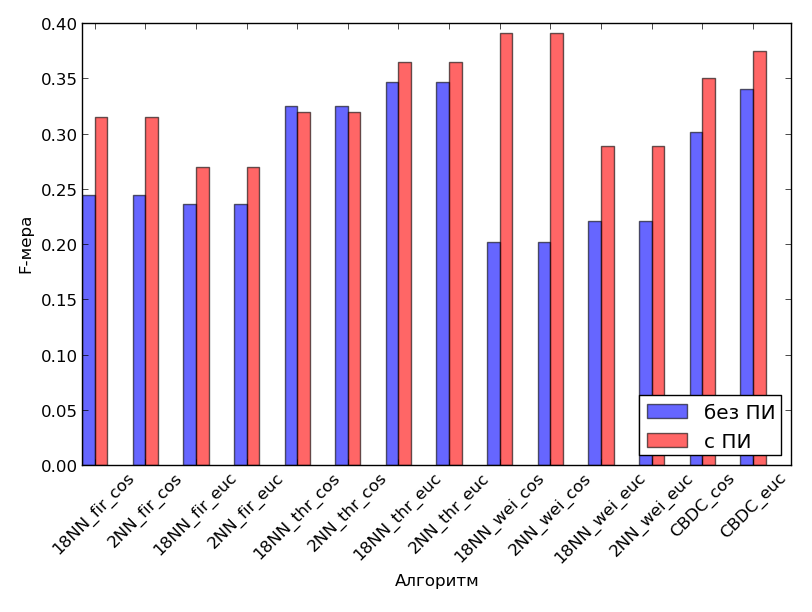
\includegraphics[width=170mm\textwidth]{perword.png}}
\caption{Гистограмма результатов запуска модификаций алгоритмов 2-NN, 18-NN и CBDC с применением перехода к исполнителю и без, perword-статистика, thresold = 0.250. ПИ \ld переход к исполнителю.}
\label{pic:perword}
\end{figure}

Как можно увидеть из таблицы \ref{tab:annotation_persong}, для первого (fir) и третьего (wei) способа фильтрации тегов алгоритмы с переходом к исполнителю показывают более высокие результаты.
В случае же второго способа фильтрации с введением порога переход к исполнителю дает сильный прирост лишь в полноте. Этот факт объясняется тем, что первый тег имеет такое значение в семантическом
веторе исполнителя, что следующий за ним в порядке убывания частоты появления среди всех треков уже не преодолевает выбранный порог. Если же увеличивать порог, то в алгоритме без перехода к исполнителю
во многих треках \emph{ни один} тег не преодолеет порог, и, как следствие, сравнивать два подхода будет уже нельзя.
Из таблицы \ref{tab:annotation_perword} видно, что при расчете статистики на тег, переход к исполнителю показывает более высокий результат и для F-меры для евлидовой метрики.

Исходя из полученных данных, можно сделать вывод, что переход к исполнителю для 2NN и для 18NN дает одинаковые результаты. Это объясняется тем, что самые основные теги, характеризующие исполнителя в целом, 
располагаются в самых первых соседях треков. Именно они и определяют первые теги в семантическом векторе исполнителя.

Стоит отметить, что лучший результат с использованием перехода к исполнителю при расчете на трек показал алгоритм 18NN(fir) с еквлидовой метрокий, а при расчете на тег \ld CBDC с косинусной метрикой.
В таблицах \ref{tab:annotation_persong} и \ref{tab:annotation_perword} соответствующие строки выделены жирным шрифтом.

\section{Эксперимент по поиску релевантных треков по тегу}

Цель данного эксперимента \ld проверить, как переход к исполнителю влияет на качество поиска релевантных треков по тегу.
Для этого мы упорядочиваем треки тестовой выборки по степени их ``принадлежности'' конкретному тегу. Чтобы оценить эту самую ``принадлежность'', в алгоритме k-NN используетя функция взвешивания.
Так как алгоритм CBDC для каждого тега возвращает расстояние $dist$ от его центра масс (см главу \ref{chapter1}) до конкретного трека, то мерой ``принадлежности'' в данном случае служит величина
$\max(dist) - dist$. Так, чем меньше расстояние, тем больше ``принадлежность''.

Для оценки качества тегирования и сравнения алгоритмов используются величины MeanAP (средняя по тегам площадь под precision-recall кривой) и MeanAROC (средняя по тегам площадь под ROC-кривой),
описанные в главе \ref{chapter1}. Подсчет производился кросс-валидацией, где $\frac{1}{10}$ часть обучающей выборки бралась для тестирования, а остальная \ld для тренировки.

В таблице \ref{tab:retrieval} приведены результаты работы алгоритмов с использованием перехода к исполнителю и без.
\begin{table}[ht]
\centering
\captionsetup{justification=centering}
\caption{Таблица с результатами применения алгоритмов 18-NN и CBDC для поиска треков по тегу с использованием перехода к исполнителю и без.}
\label{tab:retrieval}
\begin{tabular}{l c c ccc}
\hline\hline
 Алгоритм & Метрика & ПИ & MeanAP & MeanAROC
\\ [0.5ex]
    \hline

    
    & & нет&$0.431$ & $0.596$ \\[-1.5ex]
    \raisebox{1ex}{18NN} & \raisebox{1ex}{cos}
    & да &$\textbf{0.637}$ & $\textbf{0.651}$ \\[2ex]

    & & нет&$0.376$ & $0.617$ \\[-1.5ex]
    \raisebox{1ex}{18NN} & \raisebox{1ex}{euc}
    & да &$0.560$ & $0.646$ \\[2ex]

    & & нет&$0.397$ & $0.584$ \\[-1.5ex]
    \raisebox{1ex}{CBDC} & \raisebox{1ex}{cos}
    & да &$0.593$ & $0.645$ \\[2ex]

    & & нет&$0.265$ & $0.502$ \\[-1.5ex]
    \raisebox{1ex}{CBDC} & \raisebox{1ex}{euc}
    & да &$0.334$ & $0.513$ \\[2ex]

    \hline
\end{tabular}
\end{table}

Как видно из таблицы \ref{tab:retrieval}, во всех случаях переход к исполнителю дает более хорошие результаты.

Стоит отметить, что предложенный Mohamed Sordo метод CBDC в евлидовой метрике не показывает столь хороших результатов, как на CAL500.
Действительно, значение MeanAROC близко к $\frac{1}{2}$, что эквивалентно алгоритму со случайным выбором тегов.

Лучший результат показал алгоритм 18NN, соответствующие значения выделены жирным шрифтом.

\section{Выводы}

В данной главе была описана размеченная выборка с русской музыкой и описаны эксперименты. Проводилось два эксперимента \ld по сопоставлению тегов треку и по поиску релевантных треков по треку.
Было проведено сравнение методов автоматического тегирование с использованием перехода к исполнителю и без. Практически во всех случаях предложенный в данной работе метод показал более хорошие
результаты.